% !TEX root = ../master.tex
\chapter{Design and Methodology}
\label{chap:design}
TODO forcast



\section{Employed Methodology}

Preceding to the practical part of this thesis, 
the method to follow along shall be laid out here.
One suitable method is the general concept of \emph{design science research}, also known as \emph{constructive research}, 
since it involves the development and evaluation of artifacts to solve domain specific problems.
It therefore conveys a improved practical relevance in comparison to purely descriptive research methods,
while the outcomes still create scientific knowledge
\autocite[][p.~v]{dresh2015designresearch}.
The conducted research must design an artifact, such as a construct, model or method, that solves a relevant problem in a specific field, which is evaluated regarding its utility, quality and efficacy.
The performed research should be based on rigorous scientific methods and contribute to the current theoretical body of knowledge.
The conducted design process must take into account the environment it is executed in and use the available resources.
Communication of the project for both technology-oriented as well as management-oriented audiences should be present
\autocite[][p.~70]{dresh2015designresearch}.

\begin{figure}[hbt]
	\centering
	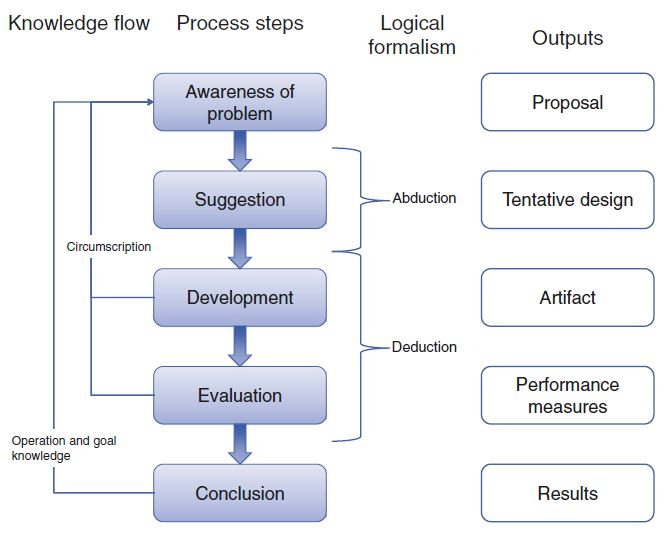
\includegraphics[width=0.8\textwidth, keepaspectratio]{resources/designscienceresearchoutputs.jpg}
	\caption{\label{fig:design:designscience} Process steps and outputs of design science research. Reprinted from \textcite[][p.~83]{dresh2015designresearch}}
\end{figure}

Figure \ref{fig:design:designscience} displays the steps that are found in the process of design science research. 
Those are the steps that guide the execution of this thesis.

TODO below are "suggestin, development and evaluation planned steps" awareness has been covered before? TODO has it?

Looking back to the original research questions (see section \vref{sec:intro:goals}) two focuses have been identified for this thesis:

\begin{itemize}
    \item Which computer vision techniques can be used to detect persons and objects within an elevator car and in front of the lift and estimate their spacial volume?
    \item How can the information acquired by a system that uses such methods constitute to the optimization of algorithms that control the movement plan for elevators?
\end{itemize}

To answer the two questions, the conducted research is therefore twofold.
The first part involves the design and experimental implementation of a system to gather passengers volume data in elevators.
The second part deals with the integration of this information into a scheduling algorithm.

TODO ref back to steps done in chapter 1- 3

TODO enums below describe suggestion and dev and evaluation

\begin{enumerate}
    \item Find a typical or actual elevator control system architecture and define the positions to integrate the necessary components for an vision system into it.
    \item Define the exact type and structure of the information that the vision system should be able to detect.
    \item Find an algorithmic approach to  passenger detection and volume estimation that is suitable to generate the required data.
    \item Match the approach with an possible hardware setup to perform tests with it.
    \item Test the proposed detection system in an real world experiment that includes  exemplary footage from within an cabin and of a lobby.
    \item Evaluate the results of the test for the functionality and effectiveness of the employed system.
\end{enumerate}

TODO

\begin{enumerate}
    \item Define a suitable elevator configuration that could possibly benefit from the information that the vision system can provide. 
    Find a typical or actual control algorithm that is used for such a configuration.
    \item Adapt the scheduling algorithm to use the additional information.
    \item Compare the two versions of the algorithm in order to determine their effectiveness regarding a suitable metric.
    A simulation is used to perform this comparison.
\end{enumerate}

TODO




general method:
design science research / constructive research
\url{https://en.wikipedia.org/wiki/Constructive_research}
\autocite[][pp.67--100]{dresh2015designresearch}, esp. fig 4.14 p.~10, 83 (steps: problem awareness, suggestion, development, evaluation, conclusion with outputs: proposal, design, artifact, performance measure, results)
but with focus on "practical utility"
therefore:
1. fuzzy sources: manual literature review that lead to fundamentals
2. theoretical body of knowlede: cullected in fundamentals
3. relevant problem: 
    - volume detectoin might hold the opportunity to further improve efficiency with the degree of usage on elevators
    - limited by 80\% oder auch 60-70\% rule \autocite[][p.~194]{unger2015aufzuege} ??, unused capacity (referece)
    - also detection of bigger items such as janitors cars, baby buggies  might be useful
4. solution construction: using engineering methods
    also:    
    - set objectives and tasks: see research questions
    - identify process model
    - select case execution
    - interview case organization
    - prepare simulation / test
    - run simulation / test
    - interpret simulation /test results
    - give feedback
5. practical relevance: interpretation of test results and considerations of marketing and economic value and need of the solution

theoretical relevance and contribution to theoretical body are not conducted

\begin{figure}[hbt]
	\centering
	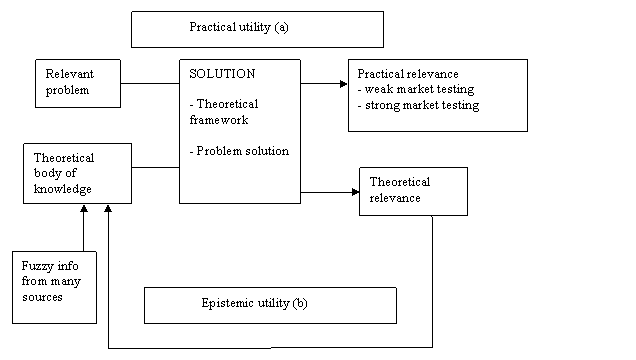
\includegraphics[width=1.0\textwidth, keepaspectratio]{resources/Rasvan_constructive_research_diagram}
	\caption{\label{fig:design:constructiveresearch} Elements of constructive research. Source:
	\url{https://en.wikipedia.org/wiki/File:Rasvan_constructive_research_diagram.gif}}
\end{figure}


come back to research questions an look onto what strategy is used to answer them

twofold:
1. design and implementation of system to gather volume data of passengers
 - find current system architecture
 - define positions to integrate new components
 - define what information should come out of the system
 (eg passenger numbers, position, tracking, volume, other objects)
 - find and choose standard algorithms for passenger detection and volume estimation in visual system (taken from fundamentals)
 - match algorithm and hardware setup possibilities
 - implement detection system
 - test detection system exemplary by filming an elevator cabin and the outside (detection system not yet influencing the elevator system)
 
2. integration of volume passenger data into existing scheduling algorithm
 - define suitable elevator configuration that can benefit from solution (taken from fundamentals) 
 - find standard algorithm for this configuration (taken from fundamentals)
 - find an integration point for the data gathered by 1.
 - compare the two algorithms effectiveness by running a simulation with the same parameters for both to check if it is even relevant to use this advanced information
 
 TODO: mapping between upper, theoretical description of method and  lower actual conduction.
 
 
 TODO rework the nexts sections according to the method defined above, also: which is design, which is implementation?

\section{Requirements}
TODO

\autocite[][]{xang2016trafficlist} has done tehe same and patentet it :(

\section{Conduction of Method}
TODO the method determines which steps to take
TODO, choose possible approach from sota

\section{Proposed Solution}
TODO next two are included?

\section{Architectural Plan}
TODO necessary? yes

\section{Algorithmic Approach}
TODO necessary? yes

\section{Validation Strategy}

TODO